\documentclass{article}
%
% surfex_doc.tex
%
% {\sc surfex} --- A Short Documentation
%

\usepackage[latin1]{inputenc}
\usepackage{latexsym}
\usepackage{amsfonts}
\usepackage{color}
\usepackage{dsfont}
\usepackage{varioref}
\usepackage{epsfig}
\usepackage[active]{srcltx}
\usepackage{hyperref}
\usepackage[english]{babel}
\usepackage{verbatim}
\usepackage{fancyhdr}

\InputIfFileExists{surfex_doc.cfg}
{\typeout{Use surfex_doc.cfg to configure the system type.}}
{\typeout{
------------ Configure for system: Linux.
}
\newcommand{\Linux}[1]{#1}\newcommand{\Windows}[1]{}
}

%\newcommand{\Linux}[1]{}\newcommand{\Windows}[1]{#1}

\newcommand{\surfex}{{\sc surfex}}
\newcommand{\attention}{\emph{Attention!}}

\newcommand{\inshell}[1]{{\\\qquad\qquad{\tt #1}}}
\newcommand{\curver}{0.89.02 }
\newcommand{\curverfile}{0\_89\_02}
\Linux{\newcommand{\INSTALL}{INSTALL\_LINUX}}
\Windows{\newcommand{\INSTALL}{INSTALL\_WINDOWS}}

\newcommand{\dZ}{{\mathds Z}}
\newcommand{\dN}{{\mathds N}}
\newcommand{\dP}{{\mathds P}}
\newcommand{\dC}{{\mathds C}}
\newcommand{\dR}{{\mathds R}}
\newcommand{\dQ}{{\mathds Q}}
\newcommand{\smcdot}{{\textup{$\cdot$}}}

\newtheorem{theorem}{Theorem}
\newtheorem{corollary}[theorem]{Corollary}
\newtheorem{remark}[theorem]{Remark}

\pagestyle{fancy}

\begin{document}

\title{{\sc surfex v.\ \curver for \Windows{Windows}\Linux{Linux/Unix}}\\
--- A Short Documentation ---}
\author{Oliver Labs}
%\address{Universit\"at des Saarlandes, Saarbr\"ucken (Germany)}

\maketitle

%\begin{abstract}
\abstract{
\noindent {\sc surfex} is a tool for interactive high quality real algebraic
surface
visualization.
It is a meta-software which combines the strenghts of several visualization
tools such as {\sc surf}, {\sc javaview}%, {\sc singsurf}
.

\noindent We also implemented a {\sc Singular} library called {\sc surfex.lib}
which enhances the quality of the visualization of {\sc surfex} using
pre-computation of the singular locus etc.

\noindent The latest version and information on {\sc surfex} and {\sc
  surfex.lib} is available from our website:
\href{http://www.surfex.AlgebraicSurface.net}{\tt
  www.surfex.AlgebraicSurface.net}.
%\end{abstract}
  \begin{center}
    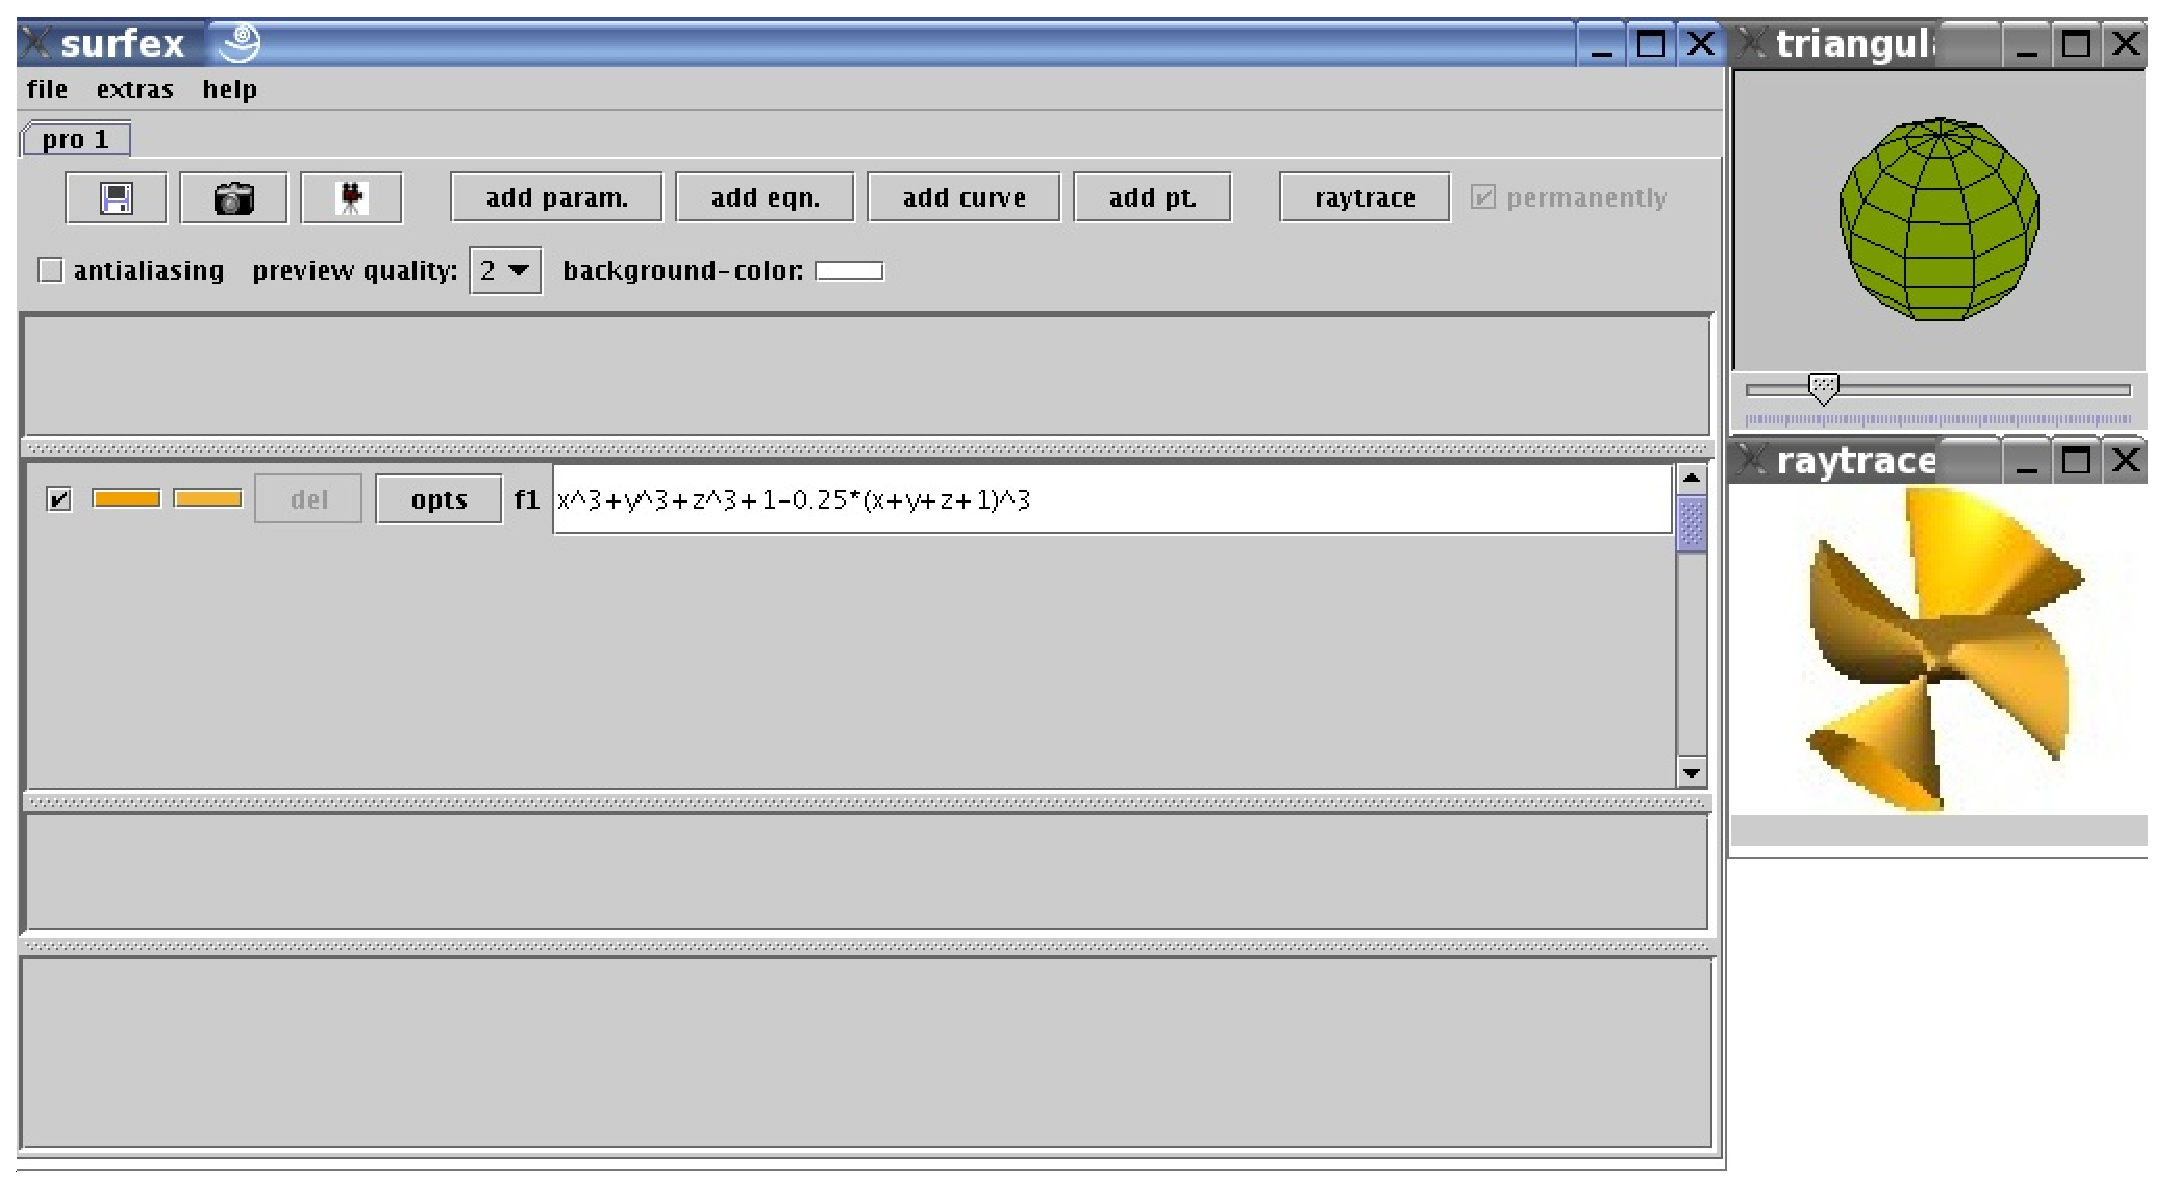
\includegraphics[width=0.8\textwidth]{surfex_simple}
  \end{center}
}

%\tableofcontents{}

% We do not want indentation at the beginning of each paragraph:
\setlength{\parindent}{0pt}
% Instead, we prefer a small vertical space between paragraphs:
\setlength{\parskip}{1ex plus 0.5ex minus 0.2ex}


%%%%%%%%%%%%%%%%%%%%%%%%%%%%%%%%%%%%%%%%%%%%%%%%%%%%%%%%%%%%%%%%%%%%%%%%%%%%%%%%
%
%
%
%%%%%%%%%%%%%%%%%%%%%%%%%%%%%%%%%%%%%%%%%%%%%%%%%%%%%%%%%%%%%%%%%%%%%%%%%%%%%%%%
\section{Getting Started}



%%%%%%%%%%%%%%%%%%%%%%%%%%%%%%%%%%%%%%%%%%%%%%%%%%%%%%%%%%%%%%%%%%%%%%%%%%%%%%%%
%
%%%%%%%%%%%%%%%%%%%%%%%%%%%%%%%%%%%%%%%%%%%%%%%%%%%%%%%%%%%%%%%%%%%%%%%%%%%%%%%%
\subsection{Download}

You can download the version \curver of our visualization software {\sc
  surfex} as one file called {\tt surfex\_\curverfile.tar.gz} from our website:
\begin{center}
\href{http://www.surfex.AlgebraicSurface.net}{\tt
  www.surfex.AlgebraicSurface.net}
\end{center}


%%%%%%%%%%%%%%%%%%%%%%%%%%%%%%%%%%%%%%%%%%%%%%%%%%%%%%%%%%%%%%%%%%%%%%%%%%%%%%%%
%
%%%%%%%%%%%%%%%%%%%%%%%%%%%%%%%%%%%%%%%%%%%%%%%%%%%%%%%%%%%%%%%%%%%%%%%%%%%%%%%%
\subsection{Prerequisites}

The current version of \surfex{}
uses the raytracer {\sc surf} as a back-end for computing the beautiful
images.
This software has to be installed on your system if you want to use
\surfex{}.
If you want to produce movies using \surfex{},
then you will also need to have the image conversion tool {\sc convert}
installed which is part of the {\sc ImageMagick} package.


%%%%%%%%%%%%%%%%%%%%%%%%%%%%%%%%%%%%%%%%%%%%%%%%%%%%%%%%%%%%%%%%%%%%%%%%%%%%%%%%
%
%%%%%%%%%%%%%%%%%%%%%%%%%%%%%%%%%%%%%%%%%%%%%%%%%%%%%%%%%%%%%%%%%%%%%%%%%%%%%%%%
\subsubsection{{\sc Java} (required)}

\surfex{} is a {\sc Java} program.
This has the advantage that it is not much work to provide the software for
many operating systems and also that it can easily be adapted to work over the
internet.

The current version of \surfex{} requires the Java Runtime Environment
(JRE), version 1.4.2 or later.
You can download it from \href{http://www.java.sun.com}{www.java.sun.com}.


%%%%%%%%%%%%%%%%%%%%%%%%%%%%%%%%%%%%%%%%%%%%%%%%%%%%%%%%%%%%%%%%%%%%%%%%%%%%%%%%
%
%%%%%%%%%%%%%%%%%%%%%%%%%%%%%%%%%%%%%%%%%%%%%%%%%%%%%%%%%%%%%%%%%%%%%%%%%%%%%%%%
\subsubsection{{\sc surf} (required)}

\Windows{
Thanks to the {\sc Singular} Team, the raytracer {\sc surf} is now also
available for Windows.
This enables us to provide \surfex{} for Windows:

The most convenient way to install {\sc surf} is to install the {\bf full
  version} of {\sc Singular for Windows} (which includes in particular {\sc
  surf}).
It uses the Linux emulation {\sc cygwin}.
The {\sc Singular} team provides their great software on their website:
\href{https://www.singular.uni-kl.de}{\tt www.singular.uni-kl.de}.
It is very easy to install; just follow the instructions.

Please, remember the directory to which {\sc Singular} installed the {\sc
  Cygwin} for later use;
at the moment, the standard seems to be {\tt c:$\backslash$cygwin}.
}

\Linux{
The canonical way to install {\sc surf} under Linux is to download the
latest version from the {\sc surf} website:
\href{http://surf.sourceforge.net}{\tt http://surf.sourceforge.net}.
After having downloaded the source code from this site, you will have to
compile and install it.
The version 1.0.5 usually compiles easily on recent Linux installations with a
recent c++ compiler.
Just follow the instructions in the {\tt \INSTALL{}} file contained in the downloaded
package.

However, for some systems there exist pre-compiled versions, see e.g.\ the
{\sc Singular} website: \href{https://www.singular.uni-kl.de}{\tt
  www.singular.uni-kl.de}.
These versions run on many Linux systems.

The standard name of the current version of the {\sc surf} binary is {\tt
  surf-1.0.5}.
Please, {\bf rename it to {\tt surf}} in order to allow \surfex{} to find it,
independantly of the current version.
}


%%%%%%%%%%%%%%%%%%%%%%%%%%%%%%%%%%%%%%%%%%%%%%%%%%%%%%%%%%%%%%%%%%%%%%%%%%%%%%%%
%
%%%%%%%%%%%%%%%%%%%%%%%%%%%%%%%%%%%%%%%%%%%%%%%%%%%%%%%%%%%%%%%%%%%%%%%%%%%%%%%%
\subsubsection{{\sc convert} (optional, for producing movies)}

For producing movies of algebraic surfaces, \surfex{} uses the great image
conversion tool {\sc convert} which is part of the {\sc ImageMagick} package.
You can download it from:
\href{http://www.imagemagick.org}{\tt www.imagemagick.org}.

\Windows{
The easiest way is to download and install a Windows binary release (do NOT
use the cygwin binary!).
Please, use the Q16-verion.
At the time of the writing of this documentation, the current version is
6.2.7-6 and the corresponding file is:
ImageMagick-6.2.7-6-Q16-windows-static.exe

Its installation is very easy; just double-click the downloaded file.
}

\Linux{
The easiest way is to download and install a binary release in the form of a
rpm package.
At the time of the writing of this documentation, the current version is
6.2.7-6 and the corresponding file is: ImageMagick-6.2.7-6.i386.rpm

To install it, type (as superuser (root)):
\inshell{rpm -i ImageMagick-6.2.7-6.i386.rpm}
}


%%%%%%%%%%%%%%%%%%%%%%%%%%%%%%%%%%%%%%%%%%%%%%%%%%%%%%%%%%%%%%%%%%%%%%%%%%%%%%%%
%
%%%%%%%%%%%%%%%%%%%%%%%%%%%%%%%%%%%%%%%%%%%%%%%%%%%%%%%%%%%%%%%%%%%%%%%%%%%%%%%%
\subsection{Install}

If you have {\sc Java} and {\sc surf} (and, optionally, {\sc convert}) installed on your
system as described above, the installation of \surfex{} should be very easy.
Just follow the steps below:

\begin{itemize}
\Windows{
\item
Copy the downloaded file {\tt surfex\_\curverfile.tar.gz} to the directory for
the temporary files of your {\sc cygwin} (if the {\sc cygwin} directory is
{\tt c:$\backslash$cygwin}, then the temporary directory will be {\tt
  c:$\backslash$cygwin$\backslash$tmp}).

\item Open a bash shell:
It is available from the Windows Start Menu via the {\sc Singular} sub-menu:
Programs $\to$ Singular CAS $\to$ Cygwin $\to$ Bash.

\item
Uncompress the downloaded file by typing the following command into the
shell:
\inshell{tar -xzvf /tmp/surfex\_\curverfile.tar.gz}
}

\Linux{
\item
Open a shell, preferably the bash shell.
This shell is available on most Linux systems.
You can start a bash by typing
\inshell{bash}\\
into a shell.

\item
Change to the directory, say {\tt /home/yourlogin/software} into which you
downloaded the file
{\tt surfex\_\curverfile.tar.gz}, e.g.\ by typing
\inshell{cd /home/yourlogin/software}\\
into a shell.

\item
Uncompress the downloaded file by typing the following command into the
shell:
\inshell{tar -xzvf surfex\_\curverfile.tar.gz}
}
\item
This should have created a directory called {\tt
  surfex\_\curverfile}.
Change to this directory by typing the following into the shell:
\inshell{cd surfex\_\curverfile}
\item
Run the {\tt \INSTALL{}} script by typing the following into the shell:
\inshell{./\INSTALL}\\
If {\tt \INSTALL{}} works well, it will produce a script
called {\tt surfex} in the current directory, and it will copy this script to
a directory which is contained in your bash path.
\item
You can now start surfex by typing:
\inshell{surfex}
\end{itemize}


%%%%%%%%%%%%%%%%%%%%%%%%%%%%%%%%%%%%%%%%%%%%%%%%%%%%%%%%%%%%%%%%%%%%%%%%%%%%%%%%
%
%%%%%%%%%%%%%%%%%%%%%%%%%%%%%%%%%%%%%%%%%%%%%%%%%%%%%%%%%%%%%%%%%%%%%%%%%%%%%%%%
\subsection{Start}

If you have installed \surfex{} correctly then you can start it by typing
\inshell{surfex}\\
into a shell.
Three windows will show up (see e.g., fig.\ \vref{fig:surfex_simple}), and a default
surface will be shown.
You can also invoke \surfex{} directly with an equation:
\inshell{surfex -e x\^{}3+y\^{}2-z\^{}2}\\
If this equation contains parenthesis then you might have to enclose the equation
in quotes: \inshell{surfex -e "(x+y)*(x-y)+z\^{}3"}\\
If you already have a \surfex{}-file, say {\tt example.sux}, then you can
open this file by typing:
\inshell{surfex example.sux}



%%%%%%%%%%%%%%%%%%%%%%%%%%%%%%%%%%%%%%%%%%%%%%%%%%%%%%%%%%%%%%%%%%%%%%%%%%%%%%%%
%
%%%%%%%%%%%%%%%%%%%%%%%%%%%%%%%%%%%%%%%%%%%%%%%%%%%%%%%%%%%%%%%%%%%%%%%%%%%%%%%%
\subsection{Examples}

The directory {\tt \curverfile} which was made during the installation process
should contain a sub-folder called {\tt examples}.

Furthermore, we will give many more examples on our website in the future,
see
\href{http://www.surfex.AlgebraicSurface.net}{\tt
  www.surfex.AlgebraicSurface.net}.



%%%%%%%%%%%%%%%%%%%%%%%%%%%%%%%%%%%%%%%%%%%%%%%%%%%%%%%%%%%%%%%%%%%%%%%%%%%%%%%%
%
%%%%%%%%%%%%%%%%%%%%%%%%%%%%%%%%%%%%%%%%%%%%%%%%%%%%%%%%%%%%%%%%%%%%%%%%%%%%%%%%
\subsection{Documentation}

The latest version of the documentation which you are currently reading is
available from our website:
\href{http://www.surfex.AlgebraicSurface.net}{\tt
  www.surfex.AlgebraicSurface.net}



%%%%%%%%%%%%%%%%%%%%%%%%%%%%%%%%%%%%%%%%%%%%%%%%%%%%%%%%%%%%%%%%%%%%%%%%%%%%%%%%
%
%%%%%%%%%%%%%%%%%%%%%%%%%%%%%%%%%%%%%%%%%%%%%%%%%%%%%%%%%%%%%%%%%%%%%%%%%%%%%%%%
\section{The Interface}


%%%%%%%%%%%%%%%%%%%%%%%%%%%%%%%%%%%%%%%%%%%%%%%%%%%%%%%%%%%%%%%%%%%%%%%%%%%%%%%%
%
%%%%%%%%%%%%%%%%%%%%%%%%%%%%%%%%%%%%%%%%%%%%%%%%%%%%%%%%%%%%%%%%%%%%%%%%%%%%%%%%
\subsection{Three Windows}

\begin{figure}[htbp]
  \begin{center}
    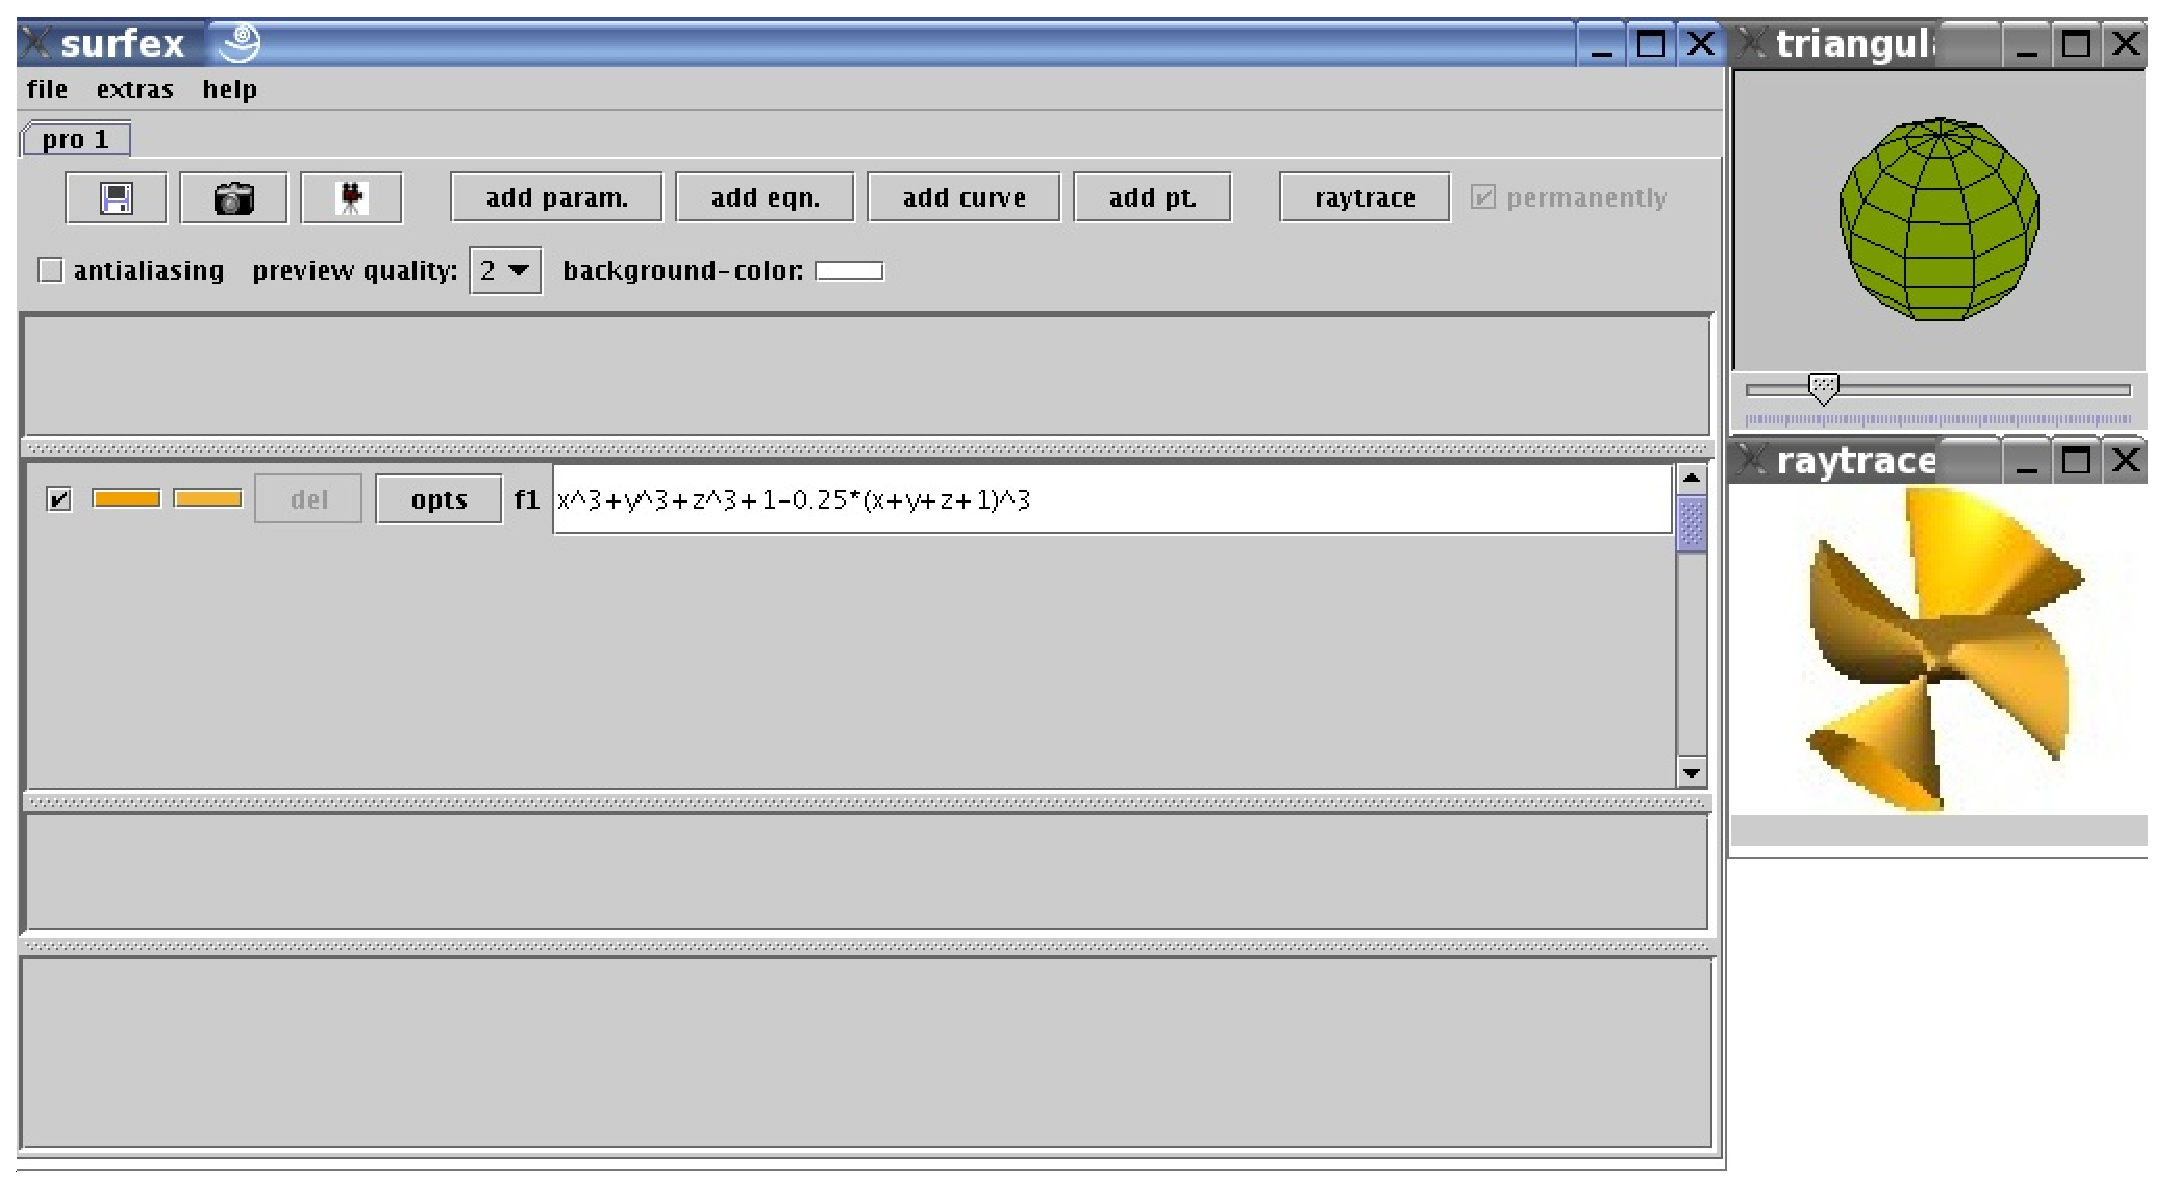
\includegraphics[width=0.8\textwidth]{surfex_simple}
    \caption{The \surfex{} interface.}
    \label{fig:surfex_simple}
  \end{center}
\end{figure}

After having started \surfex, you see three windows, entitled {\tt surfex}, {\tt
  triangulation}, {\tt raytraced surface}.

The {\tt raytraced surface} window shows a raytraced view of the surfaces
(produced using {\sc surf}).

The {\tt triangulation} window currently only shows a sphere.
By dragging the mouse on this window you can rotate the surface which is
shown in the {\tt raytraced surface} window.

The main window is the {\tt surfex} window:
here, you specify the equations and most of the other data.
We describe this in detail in the next subsection.



%%%%%%%%%%%%%%%%%%%%%%%%%%%%%%%%%%%%%%%%%%%%%%%%%%%%%%%%%%%%%%%%%%%%%%%%%%%%%%%%
%
%%%%%%%%%%%%%%%%%%%%%%%%%%%%%%%%%%%%%%%%%%%%%%%%%%%%%%%%%%%%%%%%%%%%%%%%%%%%%%%%
\subsection{The {\tt surfex} Window}


%%%%%%%%%%%%%%%%%%%%%%%%%%%%%%%%%%%%%%%%%%%%%%%%%%%%%%%%%%%%%%%%%%%%%%%%%%%%%%%%
%
%%%%%%%%%%%%%%%%%%%%%%%%%%%%%%%%%%%%%%%%%%%%%%%%%%%%%%%%%%%%%%%%%%%%%%%%%%%%%%%%
\subsubsection{The Menu}

\ \\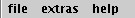
\includegraphics[scale=0.75]{surfex_menu_bar}

In the current version, the menu does not have much functionality.
Only the {\tt file} menu contains some important items:
for opening \surfex{} files, and for saving raytraced images and movies.

%%%%%%%%%%%%%%%%%%%%%%%%%%%%%%%%%%%%%%%%%%%%%%%%%%%%%%%%%%%%%%%%%%%%%%%%%%%%%%%%
%
%%%%%%%%%%%%%%%%%%%%%%%%%%%%%%%%%%%%%%%%%%%%%%%%%%%%%%%%%%%%%%%%%%%%%%%%%%%%%%%%
\subsubsection{The Project Title}

\ \\
\includegraphics[scale=0.6]{surfex_project_title}


%%%%%%%%%%%%%%%%%%%%%%%%%%%%%%%%%%%%%%%%%%%%%%%%%%%%%%%%%%%%%%%%%%%%%%%%%%%%%%%%
%
%%%%%%%%%%%%%%%%%%%%%%%%%%%%%%%%%%%%%%%%%%%%%%%%%%%%%%%%%%%%%%%%%%%%%%%%%%%%%%%%
\subsubsection{The Actions Bar}

\ \\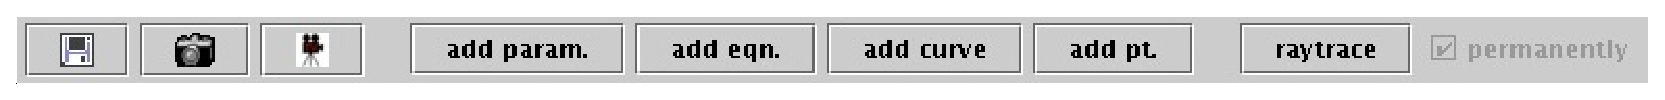
\includegraphics[scale=0.35]{surfex_actions_bar}

The main actions are performed using the actions bar.
From left to right, the buttons have the following functionalities:
\begin{itemize}
\item save the current project,
\item save the current raytraced image (in a higher resolution, if you whish),
\item save a movie, based on the current image (in a higher resolution, if you whish),
\item add a parameter to the project,
\item add an equation to the project,
\item add a curve to the project,
\item add an isolated point to the project,
\item raytrace the image once,
\item raytrace permanently; i.e., always produce new raytraced images whenever
  you have changed anything.
\end{itemize}


\subsubsection{The General Properties Bar}

\ \\
\includegraphics[scale=0.6]{surfex_general_prop_bar}

Using the general properties bar you can perform actions which do not
only have an effect on one single object, but on all varieties
simultaneously.
From left to right:
\begin{itemize}
\item antialiasing: after the computation of the raytraced image, perform an
  antialiasing (which enhances the quality, but which takes time).
\item preview-quality: 1 (best quality), \dots, 8 (lowest quality).
\item background-color: set the background color of the raytraced image.
\end{itemize}


\subsubsection{The Parameters Window}

\ \\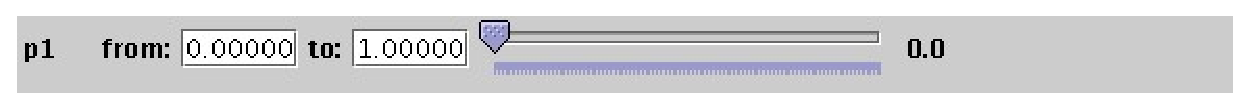
\includegraphics[scale=0.5]{surfex_parameters}

The name of the parameter (here {\tt p1}) is the leftmost information given
for each parameter.
It cannot be changed in the current version.

But you may specify the range of the parameter, and, of course, the value
of the parameter itself.
In the current version, the parameter can only be changed using the slider and
not via the keyboard.

\attention{}
Once you have changed the lower or upper bound for a
parameter by typing in some decimal number, you have to press RETURN (while
the cursor is still in the text field in which you entered the new number).


\subsubsection{The Equations Window}

\ \\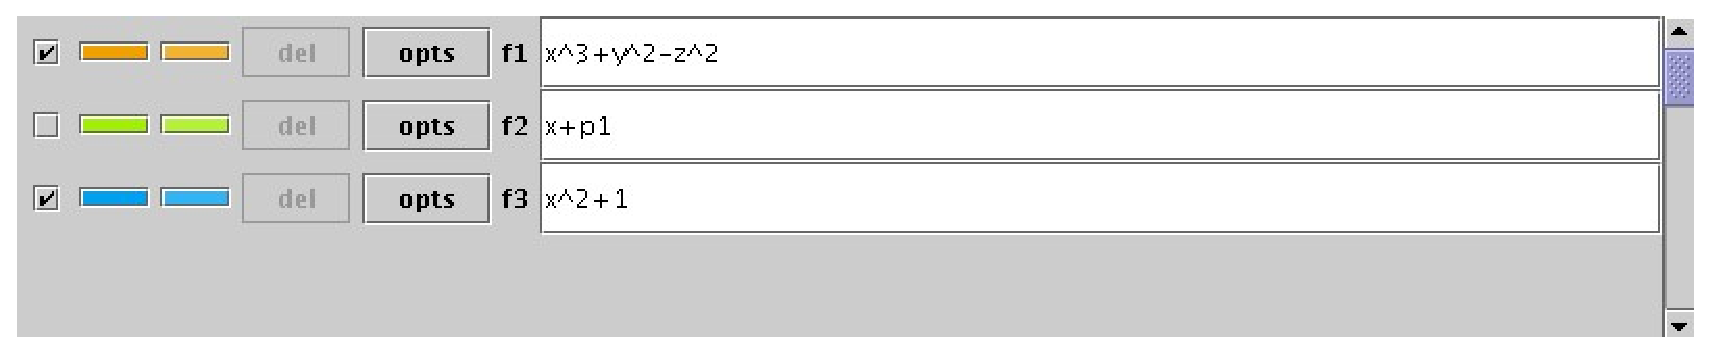
\includegraphics[scale=0.35]{surfex_equations}

A checkbox is the leftmost element for each equation.
Using this one, you can decide wether the surface should be shown in the
picture or not.

By clicking on one of the two colored buttons one can specify the inside (i.e.
looking towards the points on which the equation takes positive values) and
the outside color of the surface.

The {\tt del} button is currently disabled.

The {\tt opts} button opens an options dialogue box.
At the moment, one can only specify the transparency there (in \%).
If this is set to 100 \% then the surface is not visible at all in the
picture.

At the right of this button you can see the name of the equation.

\paragraph{Equation Syntax}

The equation itself may be entered into the big text field.
You have to give all operators explicitly: {\tt +}, {\tt -}, {\tt *},
{\tt \^{}} (i.e., e.g., {\tt 3xy} is not allowed).
As parenthesis you may use {\tt (} and {\tt )}.

Furthermore, you may include the names of the parameters (in the numerator or
denominator) and of the other equations (in the numerator).

You may even apply trigonometric functions ({\tt sin}, {\tt cos}, {\tt tan},
{\tt arccos}, {\tt arcsin}, {\tt arctan}) or {\tt sqrt} to decimal numbers or
parameters (these are actually those supported by {\sc surf}).\\
E.g., if you have two parameters {\tt p1} and {\tt p2}, and two equations {\tt
  f1} and {\tt f2}, then the equation of the third equation may e.g.\ look as
follows: {\tt cos(p1)*f1 + (sqrt(p2)+1)*f2}.

{\sc surf} also allows the usage of some functions which yield a polynomial:
\begin{itemize}
\item {\tt hesse} (produces the Hessian of a surface),
\item
  {\tt diff(p,x)}, {\tt diff(p,y)}, {\tt diff(p,z)} (the partial
  differentials, where {\tt p} is some polynomial),
\item {\tt rotate(p,v,xAxis)}, {\tt rotate(p,v,yAxis)}, {\tt
  rotate(p,v,zAxis)}, where {\tt p} is some polynomial and {\tt v} is
  some decimal number (or parameter!); in this way, you can produce your own
  non-standard rotation movie.
\end{itemize}

E.g.,
{\tt diff(f1,x)*p1 + diff(f1,y)*p2 + diff(f1,z)*p3}
is the equation of the polar of the surface {\tt f1} with respect to the point
with coordinates {\tt p1}, {\tt p2}, {\tt p3} (which can be specified using
the parameter sliders).


\subsubsection{The Curves Window}

\ \\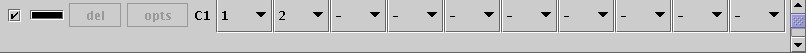
\includegraphics[scale=0.35]{surfex_curves}

Similar to the equations, you can specify if you want to see the curve or not
by using the checkbox at the left.

There is also a color button.

Each curve is then specified by giving the numbers of some equations.

\attention{}
It is important to note that the curve will be drawn on the first of the
surfaces specified.
This means in particular that the curve will only be shown if the checkbox of
this surface is checked, although its transparency can be 100 \%.
This last feature can be used to draw space curves without showing the
surface.


\subsubsection{The Solitary Points Window}

\ \\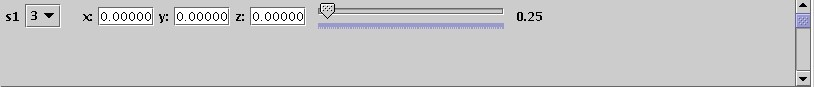
\includegraphics[scale=0.35]{surfex_points}

Solitary points can be shown as small spheres in the picture.
At the moment, their properties have to be the same as those of one of the
surfaces.
You have to select its number from the drop down list at the left.
The coordinates of the points can contain polynomials in the parameters.

The slider can be used to give the radius of the small sphere representing the
solitary point.
At the moment, all solitary points have to be represented by spheres which
have the same radius.


\end{document}
%%% Local Variables:
%%% mode: latex
%%% TeX-master: t
%%% End:
